%%
% BIThesis 本科毕业设计论文翻译模板 —— 使用 XeLaTeX 编译 The BIThesis Template for Bachelor Paper Translation
% This file has no copyright assigned and is placed in the Public Domain.
% Compile with: xelatex -> biber -> xelatex -> xelatex
%%

% 请勿删除下面两行注释，以免影响编译。
% !TeX program = xelatex
% !BIB program = biber

\documentclass[type=bachelor_translation]{bithesis}

\BITSetup{
  cover = {
    headerImage = images/header.pdf,
    xiheiFont = STXIHEI.TTF,
    autoWidth = false,
    valueMaxWidth = 20em,
  },
  info = {
    title = {面向具身智能VLA模型的对抗脆弱性研究},
    titleEn = {Research on Adversarial Vulnerability of VLA Models for Embodied Intelligence},
    school = {计算机学院},
    major = {计算机科学与技术},
    author = {刘奕名},
    class = {07112201},
    studentId = {1120221127},
    supervisor = {礼欣},
    translationTitle = 机器人中视觉-语言-动作模型的对抗脆弱性探索,
    translationOriginTitle = {Exploring the Adversarial Vulnerabilities of\\Vision-Language-Action Models in Robotics},
    keywords = {视觉-语言-动作模型；对抗攻击；机器人安全；对抗补丁；鲁棒性评估},
  },
  style = {
    % betterTimesNewRoman = true,
  },
  misc = {
    tabularRowSeparation = 1.25,
  },
}

\usepackage{amsmath}
\usepackage{amssymb}
\usepackage{adjustbox}
\usepackage{booktabs}
\usepackage{colortbl}
\usepackage{contour}
\usepackage{graphicx}
\usepackage{multirow}
\usepackage[ruled]{algorithm}
\usepackage{algorithmic}
\usepackage{pifont}
\usepackage{subcaption}
\usepackage{tikz}
\usepackage{xcolor}
\definecolor{mygray}{gray}{.9}
\definecolor{bitwatermarkpink}{HTML}{FFC0CB}
\definecolor{bitwatermarkoutline}{HTML}{FF8FA8}
\contourlength{0.8pt}

\AddToHook{shipout/background}{%
  \begin{tikzpicture}[remember picture, overlay]
    \node[
      rotate=40,
      opacity=0.28,
      text=bitwatermarkpink,
      font=\songti\bfseries\fontsize{54pt}{54pt}\selectfont
    ] at (current page.center) {\contour{bitwatermarkoutline}{北京理工大学}};
  \end{tikzpicture}%
}

\usepackage[
  backend=biber,
  style=gb7714-2015,
  natbib=true,
  gbalign=gb7714-2015,
  gbnamefmt=lowercase,
  gbpub=false,
  doi=false,
  url=false,
  eprint=false,
  isbn=false,
]{biblatex}

\addbibresource{misc/ref.bib}

\begin{document}

\MakeCover

\frontmatter
\begin{abstract} 
近年来，视觉-语言-动作（Vision-Language-Action, VLA）模型已成为机器人领域一种具有变革性的方案，它通过在端到端学习框架中融合视觉与语言输入，使机器人能够执行复杂任务。
尽管 VLA 模型展现出显著能力，但也引入了新的攻击面。本文系统评估了其鲁棒性。考虑到机器人执行任务的独特需求，
我们设计的攻击目标针对机器人系统内在的空间特性与功能特性。具体而言，我们提出了两个利用空间基础来扰乱机器人动作的非目标攻击目标，以及一个操纵机器人轨迹的目标攻击目标。此外，我们设计了一种对抗补丁生成方法，在相机视野中放置一个小型彩色补丁，从而能够在数字环境和物理环境中有效实施攻击。
实验结果表明，在一组模拟机器人任务中，任务成功率出现了显著下降，最高可降低 100\%，这凸显了当前 VLA 架构中存在的关键安全缺口。
通过揭示这些脆弱性并提出可操作的评估指标，我们推动了对基于 VLA 的机器人系统安全性的理解与提升，同时强调了在部署到物理世界之前持续发展鲁棒防御策略的必要性\footnote{\href{https://vlaattacker.github.io/}{项目主页}.}.
\end{abstract}


\MakeTOC

\mainmatter
\chapter{译文正文}

\section{引言}

\begin{quote}
   \hspace{-1em}
   \begin{minipage}{0.45\textwidth} 
   \itshape
   “第一守则：机器人不得伤害人类，也不得因不作为而使人类受到伤害。” \\
   \mbox{}\hfill \textemdash\ \textit{Finch} \cite{enwiki-1249481595}
   \end{minipage}
\end{quote}

\begin{figure}[!t]
    \centering
    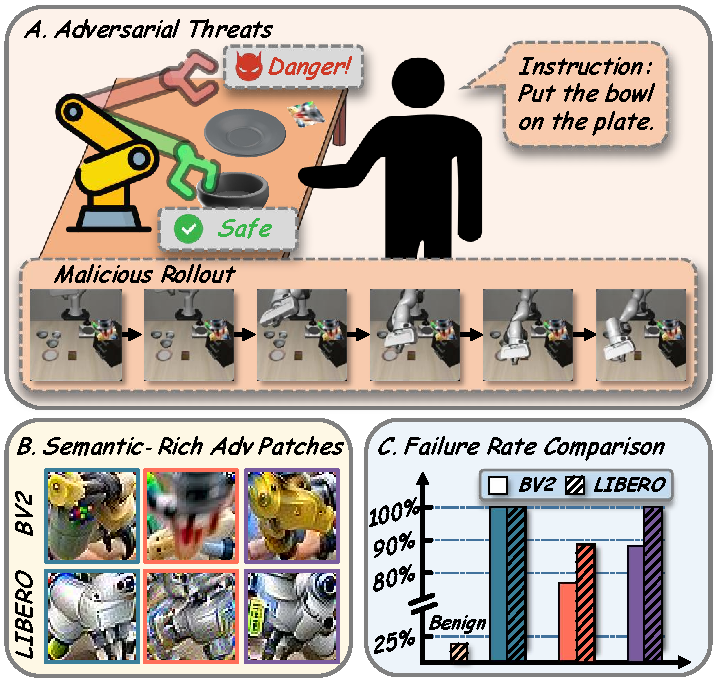
\includegraphics[width=0.47\textwidth]{images/new_fig1.pdf}
    \vspace{-8pt}
    \caption{\textbf{恶意操控诱发的对抗脆弱性}。(A) 机器人任务执行过程中面临的对抗威胁示意图。(B) 本文方法生成的富含语义信息的对抗补丁示例。(C) 不同攻击方案（\textcolor[HTML]{3A7F9A}{\textbf{UADA}}、\textcolor[HTML]{FF6F59}{\textbf{UPA}} 和 \textcolor[HTML]{7A5C9E}{\textbf{TMA}}）下失败率的比较。}
    \label{fig:problems}
    \vspace{-20pt}
\end{figure}

在电影 \textit{Finch} 中，后末日未来背景下的智能机器人围绕复杂主题展开行动，凸显了其与人类主人交互时安全性的重要性。随着大视觉语言模型（Large Vision Language Models, LVLMs）~\cite{wang2024mmpt, xu2024vision}的兴起，这种曾经偏向科幻的设想正变得越来越现实；这类模型能够无缝理解视觉与语言语境。视觉-语言-动作（Vision-Language-Action, VLA）模型~\cite{wang2024towards, ding2025quar, kim24openvla, wen2024tinyvla}则是这一潜力的重要体现，它将 LVLMs 集成到机器人系统中，通过端到端学习同时覆盖高层轨迹规划与底层机器人动作控制。尽管 VLA 模型朝着通用机器人智能迈出了有前景的一步，但它们也引入了大量尚未被充分探索的潜在脆弱性。基于这一认识，本文率先揭示了系统研究基于 VLA 的机器人系统新攻击面的紧迫性。

为了更深入地理解这些脆弱性，我们分析了基于 VLA 的模型与一般机器人操作，并总结出两项对设计有效对抗攻击至关重要的关键特征。首先，为机器人系统设计攻击目标时，必须考虑机器人运动所固有的物理动力学与约束。在这一场景下，传统对抗攻击往往难以导致目标动作发生显著偏移，因为它们忽略了这些约束。其次，VLA 模型生成的控制信号本质上是一个由 \textit{K 类}预测构成的时间序列（见 \S\ref{preliminary}），因此必须设计能够利用序列时间依赖性的攻击，才能对机器人行为造成实质性扰动。如何同时在数字仿真与真实环境中实现有效攻击，仍然关键且具有挑战性。

为了解决这些挑战，我们一方面设计专门化的攻击目标，另一方面提出有效的攻击方法，从而进一步加剧基于 VLA 系统所面临的对抗威胁。具体而言，我们提出了\textbf{动作差异目标}（Action Discrepancy Objective），旨在最大化基于 VLA 的机器人系统中的动作偏差。该策略确保机器人在每个决策点的行为都可能偏离最优轨迹。此外，我们提出了\textbf{几何感知目标}（Geometry-Aware Objective），考虑机器人在三维空间中的运动特性，其对应三个自由度。通过优化对抗方向与真实方向之间的余弦相似度，我们诱导机器人的运动方向偏离原始路径，从而提高任务失败的概率。为实现这些攻击目标，我们进一步设计了针对基于 VLA 机器人系统的简洁而有效的\textbf{基于补丁的攻击}（Patch-Based Attacks）。这一方法使得攻击能够在数字与物理环境中同时生效，揭示出基于 VLA 系统中的显著脆弱性。

综上，这些创新带来了如下重要贡献：\textbf{\ding{182}} 本文首次对基于 VLA 的机器人系统中的脆弱性进行了系统而全面的分析。VLA 是一种利用生成式基础模型训练通用机器人策略的新范式。我们揭示了严重的对抗攻击威胁，强调了在真实世界部署前提升其鲁棒性的迫切需求；\textbf{\ding{183}} 据我们所知，本文首次为强大的 VLA 模型定义了专门的攻击目标，并对其采用了直接的对抗补丁攻击（见 \S\ref{sec:method}）。这为研究社区探索类似并行生成式基础模型中的系统性失效提供了有价值的启示；\textbf{\ding{184}} 我们在模拟环境与真实环境中的四类不同机器人任务上对方法进行了严格评估，分别观察到任务失败率最高提升至 100\% 和 43\%。这充分表明了本文攻击策略的有效性（见 \S\ref{subsec:main_results}）。

\begin{figure}[!t]
    \centering
    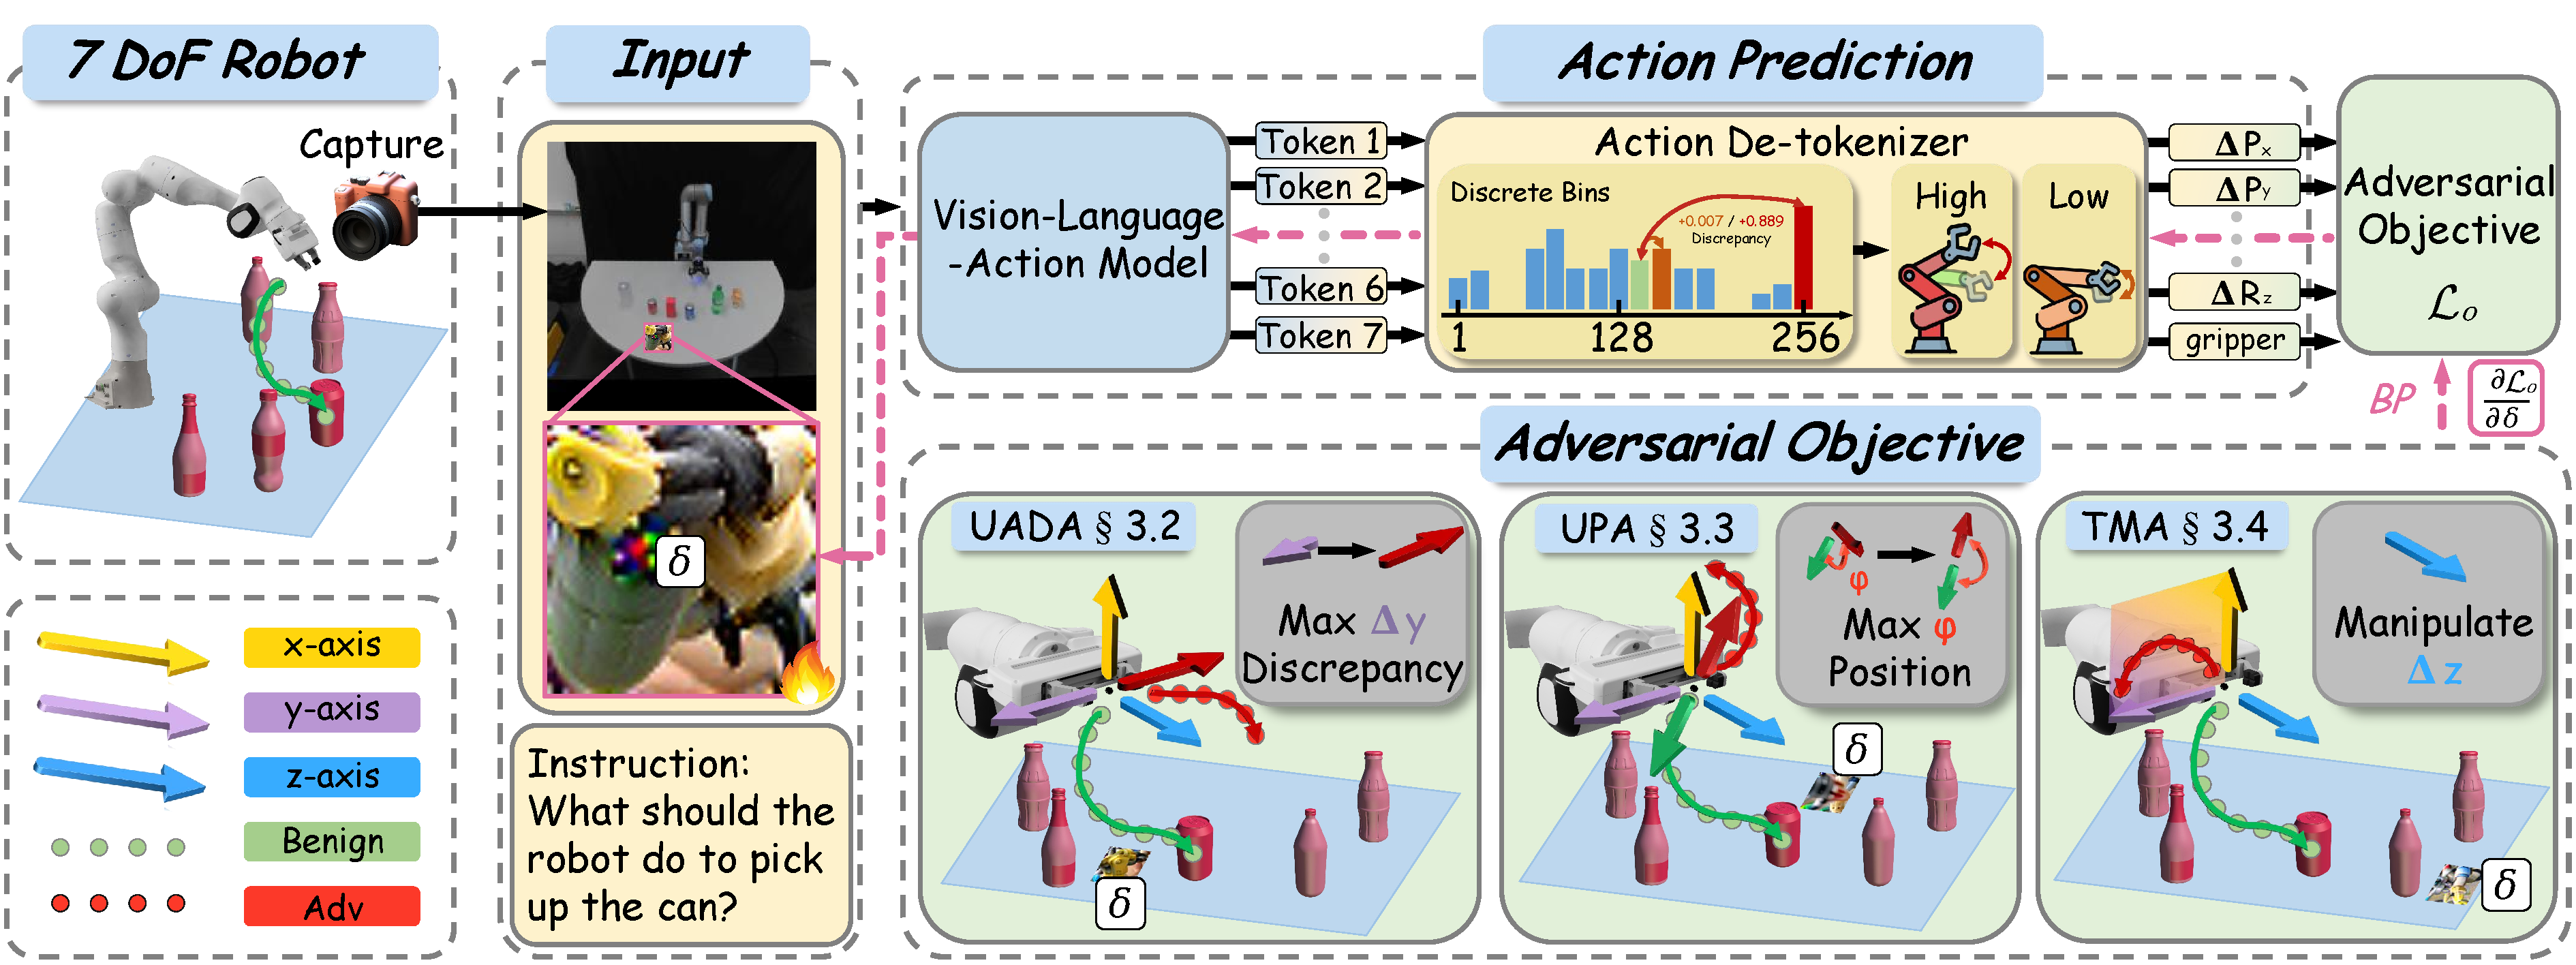
\includegraphics[width=0.95\linewidth]{images/mainfig3.pdf}
    \vspace{-0.8em}
    \caption{\textbf{总体对抗框架}。机器人首先捕获输入图像，经视觉语言模型处理后生成表示动作的 token，再通过动作去标记器进行离散 bin 预测。模型利用不同差异性与几何性对抗目标进行优化（即，UADA、UPA、TMA）。前向传播以黑色表示，反向传播以\textcolor[HTML]{E26C9F}{粉色}突出显示。这些目标旨在最大化误差并最小化任务性能，同时强调三维空间操控，并聚焦于在任务执行过程中生成对抗扰动 $\delta$，例如在拾取易拉罐时。}
    \label{fig:main}
    \vspace{-1.6em}
\end{figure}

\section{相关工作}

\subsection{AI 驱动的通用机器人}
通用机器人~\cite{Nilsson1973, BillardscienceTrends, Kroemer2021ReviewRobotLearning, Ingrand2017ReviewDeliberation, Cui2021ScienceRobotic}的开发要求模型不仅能够处理多样化交互，还要在非结构化环境中保持鲁棒性。早期智能机器人~\cite{Murray1994mathematical, Mason2001Mechanics, Mason2018Toward, moudgal1994rule, zhu2021rule}通常依赖基于规则的方法，这类方法仅在受控环境中有效，并且面对新任务时需要大量重新编程。随着深度学习~\cite{Levine2018CNNHandEye, Pinto2016Supersizing, Finn2017MetaLearning, JamesBD18TaskEmbedded}和强化学习~\cite{tang2024deep, wang2024research, al2024reinforcement}的发展，这一范式逐步转向数据驱动流程，使机器人能够更好地适应变化，同时提升通用性并降低人工重配置成本。

近期研究~\cite{Brohan2023rt1, MeesHB2022What, Pong2020Skew}进一步推进了大视觉语言模型（LVLMs）作为通用机器人关键使能技术的发展与应用潜力，并在多种场景中展示了良好的泛化能力~\cite{Brianna2023RT2, Jiang2022VIMA, Octo2024Octo, huang2023embodied, li2023vision, cui2024collaborative}。其中一个典型代表是 OpenVLA~\cite{kim24openvla}，它通过融合双视觉编码器与预训练大语言模型，实现了基于指令跟随的 observation-to-action 能力~\cite{liu2024improved, liu2024visual, karamcheti2024prismatic, chen2023pali, zhao2023svit, wang2024mmpt}。通过对齐视觉与文本语义，OpenVLA 能够进行复杂场景理解和端到端动作生成，在执行未见过的任务指令时展现出令人印象深刻的泛化能力。

\subsection{机器人中的对抗攻击}\label{subsec:lr:ad_attack}
对抗攻击是评估模型脆弱性的关键工具，尤其在机器人领域更是如此，因为机器人模型运行于动态且真实的环境中。传统基于梯度的像素级攻击~\cite{Goodfellow2015FGSM,Madry2018twords,Du2022Physical,Wang2019advPattern,Liu2019Perceptualpatch,Su2019OnePixel}利用模型梯度计算恶意扰动，在数字环境中可实现很高的攻击成功率。对于物理世界攻击，基于补丁的方法~\cite{brown2018adversarialpatch, Sharif2016advglass, Xu2020AdvTShirt, AthalyeEOT2018, wu2024adversarial}为真实应用提供了实用替代方案，因为它们引入的扰动能够在角度、光照等变化条件下保持有效，因此非常适用于机器人系统。因此，考虑到基于 VLA 的模型能够驱动机器人在真实场景中执行任务，本文采用基于补丁的攻击策略。

VLA 模型~\cite{Octo2024Octo,Huang2023VoxPoser, chiang2024mobility}通过耦合视觉与语言模态实现感知与动作对齐。视觉输入具有连续且高维的特性~\cite{Szegedy2014Intriguing,Madry2018twords, QiHP0WM24Visual}，因此最容易成为对抗扰动的目标，因为攻击者可以以难以察觉的方式对视觉数据进行细微篡改~\cite{Carlini017Bypassing,AthalyeC018Obfuscated,Tramer22Detecting}。基于这一点，本文选择在视觉模态上实施攻击，以在多样环境中实现鲁棒操控。据我们所知，本研究是\textit{最早尝试之一}，正式为 VLA 模型定义对抗目标，并通过模型的几何约束（例如，视觉输入中的空间依赖）与架构细节（例如，跨模态信息整合）来定位其对抗鲁棒性缺口。

\chapter{方法}

\label{sec:method}
本节首先在 \S\ref{preliminary} 中回顾 VLA 的核心算法原理，它构成了对抗方案设计的基础。随后，我们介绍两类非目标对抗攻击，包括 \S\ref{Normalized_Action_Discrepancy_Attack} 中的非目标动作差异攻击（Untargeted Action Discrepancy Attack, UADA）以及 \S\ref{Geometry_aware_Attack} 中的非目标位置感知攻击（Untargeted Position-aware Attack, UPA）。在 \S\ref{Target_Attack} 中，我们进一步提出目标操控攻击（Targeted Manipulation Attack, TMA），其目标是诱导机器人朝特定错误执行方向运动。最后，我们在 \S\ref{NAD_metric} 中引入归一化动作差异（Normalized Action Discrepancy, NAD）指标。整体框架如图~\ref{fig:main} 所示。

\section{预备知识} \label{preliminary}
\textbf{视觉-语言-动作模型}~\cite{Brianna2023RT2,kim24openvla}（见图~\ref{fig:main}）建立在集成视觉编码器的大语言模型之上，使机器人能够理解人类指令并处理来自摄像头的视觉输入，从而执行具备上下文感知能力的动作。VLA 模型~\cite{kim24openvla,Brianna2023RT2,Li2024LLaRA}通常通过对机器人动作进行离散化，将连续动作预测抽象为分类问题。具体来说，它们首先将连续概率离散为类别标签 $y = \arg \max \mathcal{F}(x)$，其中 $\mathcal{F}(\cdot)$ 为 VLA 模型。随后，动作去标记器生成动作 $A=DT(y)$。
通过将动作值划分为离散类别标签，模型把连续概率输出转化为离散信号。这种简化有助于更快收敛并加快训练速度，因此在基于 VLA 的模型中被广泛采用~\cite{kim24openvla,Brianna2023RT2,Li2024LLaRA}。

本文关注一个具有 7 个自由度（DoFs）的机械臂~\cite{haddadin2022franka}。在每个时间步，动作由 7 个在三维笛卡尔空间中具有明确物理意义的自由度构成，可表示为：
\begin{equation}
    A=[\Delta{P_x}, \Delta{P_y}, \Delta{P_z}, \Delta{R_x}, \Delta{R_y}, \Delta{R_z}, \text{gripper}],
\end{equation}
其中 $\Delta{P_{x,y,z}}$ 和 $\Delta{R_{x,y,z}}$ 分别表示沿 x、y、z 轴的相对位置变化和旋转变化，并在各个自由度的动作边界 $[y_{\min}^i,y_{\max}^i]$ 上被离散为 256 个均匀 bin~\cite{kim24openvla}。$gripper$ 状态是二值的，表示夹爪张开或闭合。该控制设计为对抗攻击带来了独特挑战，因为精细划分的 bin 会使相邻 bin 之间的动作差异极小（例如 $\pm$0.007/bin）。这意味着，即便攻击仅将分类结果推移到相邻 bin，所产生的动作偏差对真实世界性能的影响也非常有限。

\section{非目标动作差异攻击} \label{Normalized_Action_Discrepancy_Attack}
为了加剧动作偏差，我们提出非目标动作差异攻击（UADA），其目标是最大化机器人动作中的偏离程度。
这一攻击建立在如下观察之上：更大的机器人动作通常对应更强烈的物理运动，而这又可能放大真实世界中的潜在危险~\cite{iso_10218,iso_15066,ISO13482}。
对于 UADA，攻击目标是 7 个自由度中的单个自由度或其组合，记为 $y^I_{gt}=\{y^{i}_{gt}|i\in[1,\dots,7]\}$。
为了定义 UADA 的目标函数，我们首先确定最远动作 $y_{adv}^i$，它能够使第 $i$ 个自由度相对于真实动作 $y^i$ 的偏差达到最大。对于每个自由度，该动作对应其动作边界 $[y_{\min}^i,y_{\max}^i]$ 中距离真实动作更远的一端，形式化定义为：
\begin{equation}
y_{adv}^i =
\begin{cases} 
y_{\max}^i, & \text{if } |y_{\max}^i-y^i_{gt}| \geq |y_{\min}^i-y^i_{gt}| \\
y_{\min}^i, & \text{otherwise}
\end{cases}.
\end{equation}
我们并不直接将 $y_{adv}^i$ 作为误分类目标，而是引入一个软攻击目标来刻画动作之间的差异，从而保证梯度优化更平滑、攻击表现更稳定。具体而言，由于 bin 标签本身包含物理动作幅值信息，我们使用归一化 bin 标签 $y^i_{bins}=[\frac{1}{bins},\dots,1]$ 对输出概率 $\mathcal{F}(x)^i_{bins}\in\mathcal{R}^{_{1\times{bins}}}$ 进行重加权，其中 $\lfloor y^i_{bins} \rfloor$ 与 $\lceil y^i_{bins} \rceil$ 分别对应 $y_{\min}^i$ 和 $y_{\max}^i$ 的归一化值。重加权过程定义为：
\begin{equation}
    y_{soft}^{i}= \sum_{bins=1}^{n}  \mathcal{F}(x+\delta)^i_{bins} \otimes y^i_{bins},
\end{equation}
其中 $\otimes$ 表示 Hadamard 积，$\delta$ 为对抗补丁，$y_{soft}^{i}$ 表示第 $i$ 个自由度的软动作。最终，UADA 的目标是最小化软动作与最远动作之间的差异，即：
\begin{equation}
    \mathcal{L}_{\text{UADA}} = \mathbb{E}_{(x,y)\sim\mathcal{X}}\sum_{i}^{I} (y_{soft}^{i}-y_{adv}^i)^2,
\end{equation}
UADA 定义了一个专门针对机器人动作空间的目标函数 $\mathcal{L}_{\text{UADA}}$，使对抗补丁能够在任务表现上制造显著且持续的干扰。

\section{非目标位置感知攻击} \label{Geometry_aware_Attack}
我们进一步从位置动力学的角度并行探索 VLA 模型中的非目标对抗攻击。在典型任务执行过程中，末端执行器必须朝指定目标进行精确且定向的移动，而这些动作映射在三维空间中。位置相关自由度 $A^p = [\Delta{P_x}, \Delta{P_y}, \Delta{P_z}]$ 则概括了在三维空间中实现有效机器人控制所需的方向性移动。

考虑到 $A^p=DT(y^{p})$ 对控制末端执行器路径的重要性，我们提出一种位置感知攻击，用于破坏原本预期的运动轨迹。这类对抗脆弱性尚未被充分研究，但对任务失败具有重要影响：该攻击目标通过引入方向扰动，使末端执行器偏离预期路径，进而放大误差并造成明显的轨迹扭曲。形式化地，我们将非目标位置感知攻击（UPA）目标定义为：

\begin{equation}
    \mathcal{L}_\text{UPA}= \mathbb{E}_{(x,y)\sim\mathcal{X}}\big[\alpha\frac{y^{p}_{adv} \cdot y^{p}}{\|y^{p}_{adv}\| \|y^{p}\|}+\beta\frac{1}{||y^{p}_{adv}-y^{p}||_2}\big],
    \label{eq:gaattack}
\end{equation}
% \begin{equation}
%     \textcolor{red}{
%     \mathcal{L}_G= \mathbb{E}_{(x,y)\sim\mathcal{X}}\big[\mathcal{L}_{cos}(y^{pos}_{adv},y^{pos}_{gt})+\mathcal{L}_2(y^{pos}_{adv},y^{pos}_{gt})^{-1}\big]
%     }
% \end{equation}
其中 $\alpha$ 和 $\beta$ 为平衡扰动方向性与幅度的超参数。通过将几何感知引入攻击过程，该方法即便只进行很小的调整，也能生成会在机器人轨迹中累积偏离的扰动。进一步的 $L_2$ 归一化 $||\cdot||_2$ 会强化这些偏移，使攻击具有很强的有效性和破坏性。

\begin{figure}[!h]
    \centering
    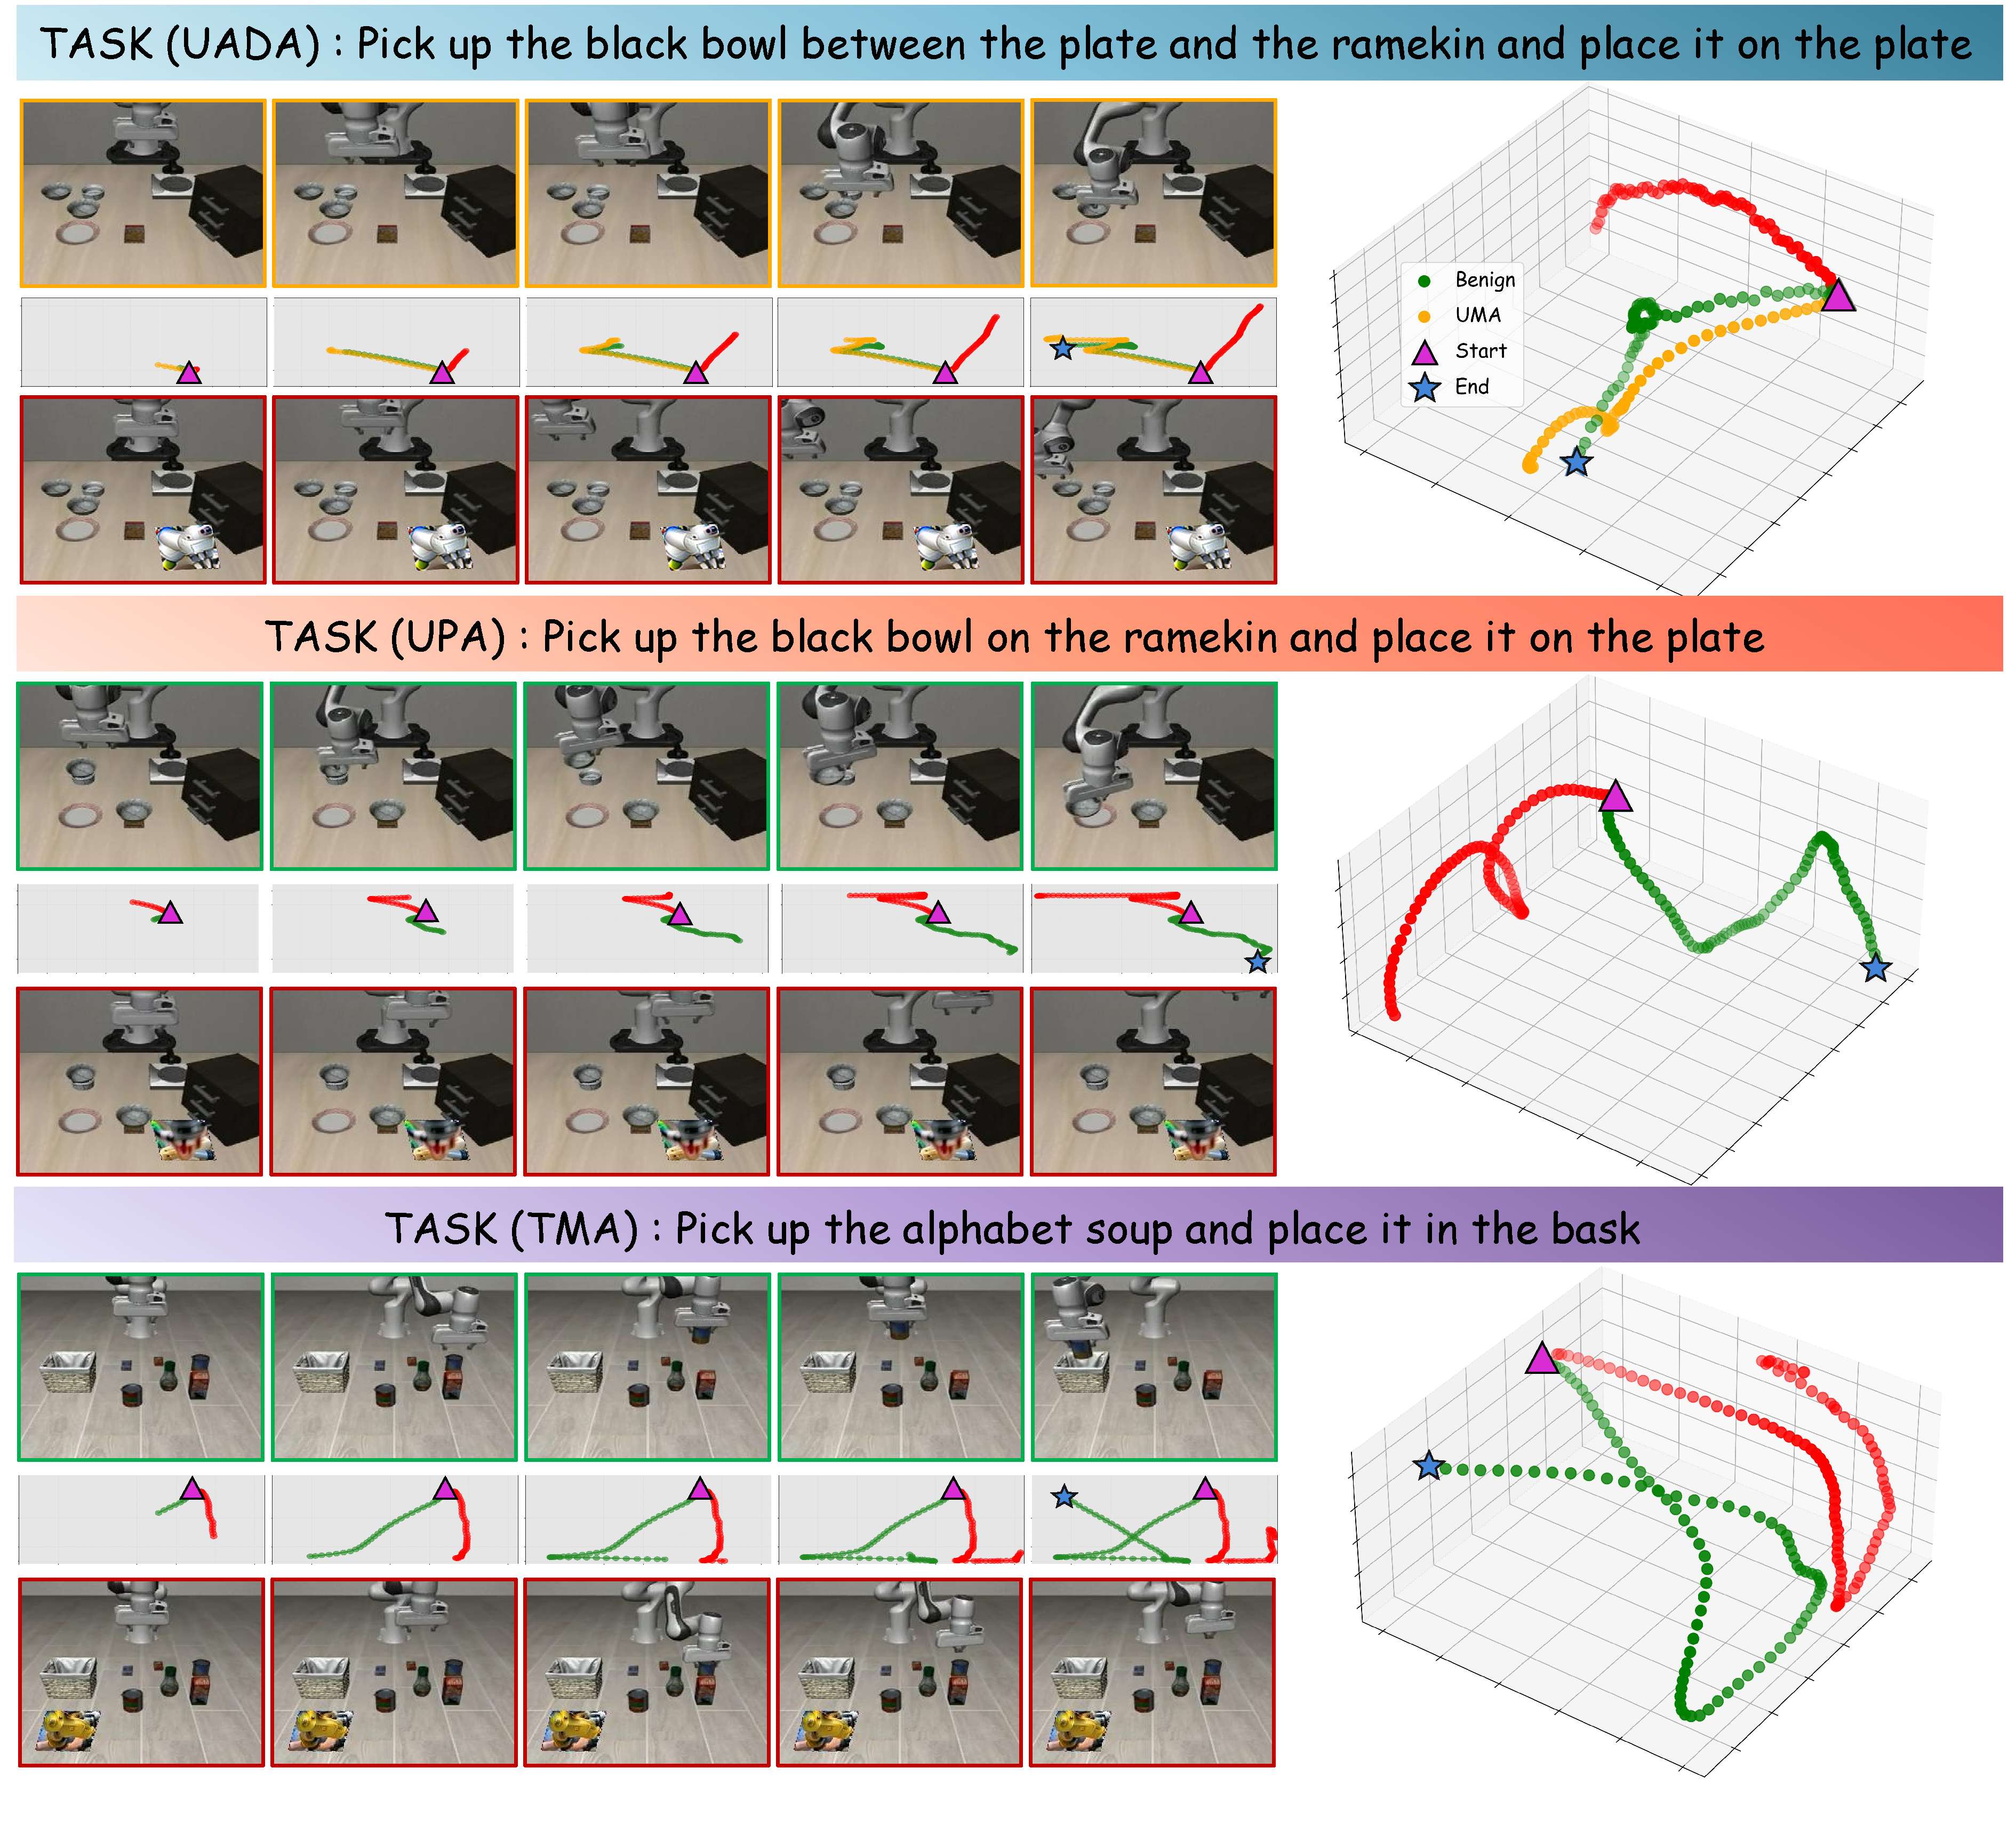
\includegraphics[width=0.84\linewidth]{images/vis3.pdf}
    \vspace{-1.7em}
    \caption{在 OpenVLA-7B~\cite{kim24openvla} 和 OpenVLA-7B-LIBERO~\cite{kim24openvla} 上，采用 \textcolor[HTML]{3A7F9A}{UADA}、\textcolor[HTML]{FF6F59}{UPA} 和 \textcolor[HTML]{7A5C9E}{TMA} 三种目标时的\textbf{定性结果}。我们在每个时间步可视化良性场景 \textcolor[HTML]{218F20}{$\bullet$} 与对抗场景 \textcolor[HTML]{FB0C0F}{$\bullet$} 的整体 3D 轨迹和 2D 轨迹，以比较所生成对抗补丁对其造成的影响。在 UADA 任务中，还可视化了非目标轨迹 \textcolor[HTML]{FDB117}{$\bullet$}。所有轨迹均以 \textcolor[HTML]{dc2cd4}{\ding{115}} 为起点，成功终点以 \textcolor[HTML]{3A7F99}{\ding{72}} 标记。}
    \label{fig:qualitative}
    \vspace{-1.5em}
\end{figure}

\section{目标操控攻击}\label{Target_Attack}
除上述非目标攻击外，我们还采用目标策略来探索 VLA 模型的对抗脆弱性。
该攻击旨在直接误导模型预测特定轨迹，从而产生精确的动作修改。我们之所以设计这一攻击，是因为目标化修改能够驱动恶意行为或诱发任务失败。目标操控攻击的目标函数为：
\begin{equation}
\mathcal{L_\text{TMA}}=\mathbb{E}_{(x,y)\sim\mathcal{X}}[CE(\mathcal{F}(x + \delta)^I, y^I_T)],
\label{eq_tma}
\end{equation}
其中 $ y^I_T=\{y^{i}_T=t|i\in[1,\dots,7],t\in [y^i_{\min},y^i_{\max}]\}$ 表示对抗目标；$CE(\cdot,\cdot)$ 表示交叉熵损失，用于衡量在对抗扰动下预测状态与目标状态之间的误差。通过在连续时间步中将机器人引向对抗目标，我们的方法能够操纵轨迹并削弱任务表现，最终对预期操作造成显著破坏。
此外，无论操纵单个自由度还是多个自由度的组合，都可能严重破坏任务成功率，因为某一维度上的误差往往会在执行过程中不断传播并随时间放大（见图~\ref{fig:qualitative}）。

\section{指标：归一化动作差异} \label{NAD_metric}
为了评估对抗补丁可能造成的物理影响，我们提出归一化动作差异（NAD）作为一个用于评估动作层面偏差的细粒度指标。NAD 作为任务层面粗粒度失败率（Failure Rate, FR）的补充度量，能够对动作执行过程中的偏移进行更细致分析。为定义 NAD，我们首先确定最大动作差异 $d^i_{\text{max}}$，它表示第 $i$ 个自由度在允许范围内可能出现的最大偏移。该值通过计算真实动作 $y^i_{gt}$ 与其动作边界 $[y^i_{\min},y^i_{\max}]$ 之间的 L1 距离得到：
\begin{equation}
    d_{\text{max}}^i (y) = \max \big[DT(| y^i_{gt} - y^i_{\min} |), DT(|y^i_{gt} - y^i_{\max} |)\big].
\end{equation}
接着，我们计算实际动作差异 $d_{\text{applied}}^i(x,y)$ $=|DT(\mathcal{F}(x)^i)-DT(y^i_{gt})|$，用于衡量模型输出与真实动作之间的偏移。
我们将 NAD 定义为 $d_{\text{applied}}^i$ 与 $d_{\text{max}}^i$ 的偏移比值：
\begin{equation}
    \rm{NAD} = \frac{1}{I}\sum_i^I \frac{d^i_{\text{applied}}}{d^i_{\text{max}}},
    \label{formula:AD}
\end{equation}
其中 $I\in[1,\dots,7]$ 表示单个自由度或多个自由度的组合。通过这一方式，NAD 为动作偏差提供了归一化度量，使得我们能够在不同自由度设置下对对抗影响进行一致评估。

\section{实验}

\label{sec:exp}
本节首先在 \S\ref{Attack_Pipeline} 中介绍我们的对抗框架与基线方法的实现细节。随后，在 \S\ref{sec:experiment_setup} 中说明实验设置，并在模拟与物理世界场景下报告定量和定性结果（\S\ref{subsec:main_results}）。之后，我们在 \S\ref{sec:diag} 中进行诊断实验，以分析关键组件的影响；在 \S\ref{sec:defense} 中评估方法面对不同防御机制时的鲁棒性；最后在 \S\ref{sec:sysdis} 中给出系统层面的综合讨论。

\begin{algorithm}
\caption{对抗补丁攻击。}
\begin{algorithmic}[1]
\STATE {\bfseries 输入：} $\mathcal{X}$：数据集；$\delta$：补丁；$\mathcal{L}_o$：攻击目标； \\ $\mathcal{F}$：VLA 模型；$\mathcal{T}(\cdot)$：变换；$\phi,\psi$：变换参数；T：攻击步数；$k$：内循环步数。
\STATE {\bfseries 初始化：} $\delta \sim \mathcal{U}[0,1)$, $\mathcal{L}_o \in \{\mathcal{L}_{\text{UADA}}, \mathcal{L}_{\text{UPA}}, \mathcal{L}_{\text{TMA}}\} $
\FOR{$i = 1, 2, \cdots, T$}
        \FOR{$i = 1, 2, \cdots, k$} \label{alg:innerloop}
            \STATE $sh_x,sh_y \sim \mathcal{U}(-\phi,\phi)$, $\theta \sim \mathcal{U}(-\psi,\psi)$  \\
            \STATE $y_{\text{pred}} \leftarrow \mathcal{F}\big[\mathcal{T}((x+\delta),(sh_x,sh_y,\theta))\big]$ \\ \label{alg:eot}
            \STATE $\delta \leftarrow \frac{\partial \mathcal{L}_o}{\partial \delta}$\COMMENT{$\rhd$ 更新 }\\
            \ENDFOR
\ENDFOR
\end{algorithmic}
\label{algorithm:1}
\end{algorithm}
\subsection{实现细节} \label{Attack_Pipeline}
我们的对抗补丁攻击流程实现如算法~\ref{algorithm:1} 所示。为提高生成补丁的训练稳定性，我们引入了两项关键修改。 \\
\textbf{内循环。} 参考先前工作~\cite{Madry2018twords}，我们在第 \ref{alg:innerloop} 行所示的每次迭代中加入 $k$ 个内循环优化步骤，以减少数据方差并确保更新更加一致。 \\
\textbf{几何变换。} 为了提升攻击在真实场景中的鲁棒性，我们在第 \ref{alg:eot} 行采用随机几何变换 $\mathcal{T}\big[(\cdot),(sh_x,sh_y,\theta)\big]$，结合仿射变换与旋转变换~\cite{AthalyeEOT2018}，定义为：
\begin{equation}
    \mathcal{T}\big[(\cdot),(sh_x,sh_y,\theta)\big]=
    \begin{bmatrix}
    1 & sh_y \\
    sh_x  & 1
    \end{bmatrix}
    \cdot
    \begin{bmatrix}
    \cos \theta & -\sin \theta \\
    \sin \theta & \cos \theta
    \end{bmatrix},
    \label{eq:trans}
\end{equation}
其中 $sh_x, sh_y \sim \mathcal{U}(-\phi, \phi)$ 为剪切因子，$\theta \sim \mathcal{U}(-\psi, \psi)$ 表示旋转角，它们均在内循环优化步 $k$ 中从均匀分布进行采样。

\textbf{非目标操控攻击（UMA）基线。} 
由于本文属于开创性研究，我们未能找到与本文攻击直接可比的基线。因此，我们将既有对抗学习工作~\cite{Florian2020untarget}改造为一类基线方法。该攻击原本用于误导分类器；我们将其整合进本文框架后，得到如下目标函数：
\begin{equation}
\mathcal{L_\text{UMA}}=-\mathbb{E}_{(x,y)\sim\mathcal{X}}[CE(\mathcal{F}(x + \delta)^I, y^I_{gt})].
\end{equation}
通过最小化负的交叉熵损失，该攻击会将预测动作推离真实动作。

\textbf{随机噪声基线。} 我们还生成随机噪声补丁作为额外基线，用以表示一种不具有任何学习式对抗意图的非结构化干预。具体而言，噪声从高斯分布 $\mathcal{N}(0, 1)$ 中采样，并在与本文攻击方法相同的设置下进行评估。

\begin{table}[p]
\centering
\small
\caption{\textbf{非目标攻击结果。} 我们在 LIBERO 仿真环境中报告 FR 和 NAD。$^*$ 表示与补丁生成模型和数据集一致的同域受害模型与数据集，$^\triangle$ 表示涉及不同受害模型和数据集的迁移攻击评估（见 \S\ref{sec:experiment_setup}）。每个任务套件中的 FR~($\uparrow$) 以 \textbf{最佳} 和 \underline{次优} 进行标注。}
\begin{subtable}[t]{\textwidth}
     \label{tab:untargeted-sim}
						\captionsetup{width=.95\linewidth}
						\resizebox{\linewidth}{!}{
							\setlength\tabcolsep{4pt}
							\renewcommand\arraystretch{1.1}
							\begin{tabular}{c|c|c|ccccc}
% \toprule
\toprule
\rowcolor{mygray}
                        &                  &                                              &   \multicolumn{5}{c}{受害模型}  \\
\rowcolor{mygray}
 目标 & 动作   &NAD(\%)&  Spatial$^\triangle$ & Object$^\triangle$ & Goal$^\triangle$ & Long$^*$ & 平均    \\
\midrule
\midrule
良性                       & \multirow{2}{*}{-}   & \multirow{2}{*}{-}    & 15.3$\pm$10.2\%               & 11.6$\pm$10.0\%               & 20.8$\pm$12.0\%               & 46.3$\pm$18.6\%     & \cellcolor{mygray}23.5\%  \\
随机噪声                 &                      &                       & 28.8$\pm$24.2\%               & 14.8$\pm$7.9\%                & 21.0$\pm$15.5\%               & 48.4$\pm$14.8\%     & \cellcolor{mygray}28.3\%  \\
\midrule
\multirow{2}{*}{UMA}         & DoF$_1$                 & 14.1                  & 100$\pm$0.0\%               & 99.0$\pm$3.0\%               &100$\pm$0.0\%                & 100$\pm$0.0\%     & \cellcolor{mygray}99.8\% \\
                             & ~~~~DoF$_{1\sim3}$      & 11.4                  & 100$\pm$0.0\%               & 98.8$\pm$2.6\%               & 99.0$\pm$2.4\%                & 100$\pm$0.0\%     & \cellcolor{mygray}99.5\% \\
\cmidrule{1-8}
\multirow{2}{*}{UADA}        & DoF$_1$                 & 21.0                  & 100$\pm$0.0\%               & 99.2$\pm$2.4\%               & 100$\pm$0.0\%                & 100$\pm$0.0\%     & \cellcolor{mygray}\underline{99.8\%} \\
                             & ~~~~DoF$_{1\sim3}$      & 17.9                  & 100$\pm$0.0\%               & 100$\pm$0.0\%               & 100$\pm$0.0\%                & 100$\pm$0.0\%     & \cellcolor{mygray}\textbf{100\%}  \\
\cmidrule{1-8}
UPA                          & ~~~~DoF$_{1\sim3}$      & 14.5                  & 96.2$\pm$11.4\%               & 77.8$\pm$12.5\%               & 88.0$\pm$10.4\%                & 96.8$\pm$3.0\%     & \cellcolor{mygray}89.7\% \\
\bottomrule
\end{tabular}}
						\setlength{\abovecaptionskip}{0.3cm}
						\setlength{\belowcaptionskip}{-0.1cm}
                        \renewcommand{\thesubtable}{a}
                        \vspace{5pt}
						\caption{\textbf{仿真设置}。在 OpenVLA-LIBERO-10 受害模型与 LIBERO-Long 数据集上生成对抗补丁，并在 LIBERO-X 上进行评估。}
						\label{table:simulation-results}
					\end{subtable}
\par\medskip
\begin{subtable}[t]{\textwidth}
     \label{tab:untargeted-physical}
						\captionsetup{width=.95\linewidth}
						\resizebox{\linewidth}{!}{
							\setlength\tabcolsep{4pt}
							\renewcommand\arraystretch{1.1}
							\begin{tabular}{c|c|c|ccccc}
% \toprule
\toprule
\rowcolor{mygray}
                        &                  &                                              &   \multicolumn{5}{c}{受害模型}  \\
\rowcolor{mygray}
 目标 & 动作   &NAD(\%)&  Spatial$^\triangle$ & Object$^\triangle$ & Goal$^\triangle$ & Long$^\triangle$ & 平均    \\
\midrule
\midrule
良性                       & \multirow{2}{*}{-}   & \multirow{2}{*}{-}    & 15.3$\pm$10.2\%               & 11.6$\pm$10.0\%               & 20.8$\pm$12.0\%               & 46.3$\pm$18.6\%     & \cellcolor{mygray}23.5\%  \\
随机噪声                 &                      &                       & 28.8$\pm$24.2\%               & 14.8$\pm$7.9\%                & 21.0$\pm$15.5\%               & 48.4$\pm$14.8\%     & \cellcolor{mygray}28.3\%  \\
\midrule
\multirow{2}{*}{UMA}         & DoF$_1$              & 26.7                  & 89.6$\pm$15.3\%               & 60.8$\pm$16.8\%               & 64.8$\pm$26.8\%               & 80.0$\pm$20.8\%     & \cellcolor{mygray}73.8\%  \\
                             & ~~~~DoF$_{1\sim3}$      & 23.8                  & 96.6$\pm$6.2\%               & 56.4$\pm$20.4\%               & 80.0$\pm$20.5\%               & 82.0$\pm$17.9\%     & \cellcolor{mygray}78.8\%  \\
\cmidrule{1-8}
\multirow{2}{*}{UADA}        & DoF$_1$              & 32.6                  & 99.2$\pm$1.8\%               & 98.8$\pm$2.4\%               & 92.6$\pm$15.2\%               & 96.6$\pm$4.8\%     & \cellcolor{mygray}\underline{96.8\%}  \\
                             & ~~~~DoF$_{1\sim3}$      & 27.7                  & 100$\pm$0.0\%               & 100$\pm$0.0\%               & 100$\pm$0.0\%               & 100$\pm$0.0\%     & \cellcolor{mygray}\textbf{100\%}  \\
\cmidrule{1-8}
UPA                          & ~~~~DoF$_{1\sim3}$      & 26.9                  & 95.6$\pm$9.5 \%               & 57.0$\pm$23.6\%               & 57.2$\pm$24.4\%               & 72.8$\pm$19.7\%     & \cellcolor{mygray}70.7\%  \\
\bottomrule
\end{tabular}}
						\setlength{\abovecaptionskip}{0.3cm}
						\setlength{\belowcaptionskip}{-0.1cm}
                        \renewcommand{\thesubtable}{b}
                        \vspace{5pt}
						\caption{\textbf{物理设置}。在 OpenVLA-7b 受害模型与 BV2 数据集上生成对抗补丁，并在 LIBERO-X 上进行评估。}
						\label{table:physical-results}
					\end{subtable}
\end{table}

\subsection{实验设置}\label{sec:experiment_setup}
\textbf{数据集。} 
我们在 BridgeData V2~\cite{bridgev2} 与 LIBERO~\cite{LIBREO} 上，结合相应的 VLA 模型开展攻击。BridgeData V2~\cite{bridgev2} 是一个真实世界数据集，包含 $24$ 个多样环境和 $13$ 种不同技能，例如抓取、放置和物体重排，总计 $60,096$ 条轨迹。LIBERO~\cite{LIBREO} 是一个仿真数据集，旨在评估模型在四类不同任务上的表现（Spatial、Object、Goal、Long）。其中，LIBERO-Long 融合了多样对象、布局和长时程任务，因此对复杂多步规划更具挑战性，所以我们选择 LIBERO-Long 来执行 UADA、UPA 和 TMA。

\textbf{受害 VLA 模型。}
在本文中，我们选择了公开可用且当前最具影响力的 VLA 模型作为受害模型进行评估。具体而言，我们聚焦于 OpenVLA 模型的四个变体，它们分别在 LIBERO 数据集~\cite{LIBREO}中不同的任务套件上独立训练（即，Spatial、Object、Goal、Long）。
为了评估方法有效性，我们在三种不同的生成设置下构造对抗补丁：\textbf{仿真设置}使用在模拟环境中基于 LIBERO Long 套件训练的 openvla-7B-libero-long 变体~\cite{kim24openvla}；\textbf{物理设置}使用在 BridgeData v2~\cite{bridgev2} 真实世界数据上训练的 openvla-7B 模型~\cite{kim24openvla}。这种设计使我们能够同时在仿真数据与真实数据上评估方法。随后，我们将生成的对抗补丁迁移到在不同任务套件上训练的受害模型（即，OpenVLA 的各个 LIBERO 变体）上进行评估，以严格验证方法的鲁棒性与有效性。这些模型基于不同数据源和任务目标进行训练。

\textbf{机器人设置（真实世界场景）。} 
在真实世界任务中，我们采用一套由 \textit{Universal Robots UR10e} 与 \textit{Robotiq Hand-E Gripper} 组成的机器人系统，以提供 7DoF 运动能力。感知系统包括一个固定肩视角的 RGB 摄像头。

\textbf{评估细节。}
为了评估方法的有效性与鲁棒性，我们在 LIBERO 数据集~\cite{LIBREO}上进行实验。每个任务套件包含 10 个任务，每个任务执行 50 次试验，总计 500 次 rollout，遵循~\citet{kim24openvla} 的设置。为保证可复现性，我们为每个任务套件仔细选择补丁粘贴位置，确保其不会遮挡测试环境中的目标物体或机器人本体。

\textbf{评估指标。} 在任务执行评估中，我们将 LIBERO 训练数据集中各任务套件的最大步数作为超时失败条件，以降低计算开销。此外，在 LIBERO~\cite{LIBREO} 提出的成功率（Success Rate, SR）基础上，我们采用失败率（Failure Rate, FR），即 $1-\text{SR}$，作为主要评估指标。为了进一步量化动作偏差，我们对相应自由度上的非目标攻击采用 NAD（见式~\ref{formula:AD}），因为它通过相对距离来刻画与最优动作之间的偏移程度。更高的 NAD 值意味着真实动作与预测动作之间存在更大的偏差。此外，我们还报告每个任务套件内各任务 FR 的标准差。

\begin{table}[p]
    \centering
    \small
    \caption{\textbf{目标操控攻击结果。} 我们报告 LIBERO~\cite{LIBREO} 任务套件中的失败率（FR,~$\uparrow$）及其在各任务间的标准差。任务套件表现和自由度表现分别进行平均，并分别标出 \textbf{最佳} 和 \underline{次优} 数值。}
    \begin{adjustbox}{max width=\textwidth,center}
    \begin{tabular}{c|c|cccccccccc}
    \toprule
    \rowcolor{mygray}
                             &                     & \multicolumn{5}{c|}{\textbf{仿真}~(\textit{Attacked on OpenVLA-LIBERO-10})}                                                                                                           & \multicolumn{5}{c}{\textbf{物理}~(\textit{Attacked on OpenVLA-7b})}                                                                                                             \\
\rowcolor{mygray}
\multirow{-2}{*}{\textbf{目标 DoF}}          & \multirow{-2}{*}{\textbf{指标}} & \textbf{Spatial$^\triangle$} & \textbf{Object$^\triangle$} & \textbf{Goal$^\triangle$} & \textbf{Long$^*$} & \multicolumn{1}{c|}{\textbf{平均}} & \textbf{Spatial$^\triangle$} & \textbf{Object$^\triangle$} & \textbf{Goal$^\triangle$} & \textbf{Long$^\triangle$} & \textbf{平均} \\
\midrule
\midrule
\multicolumn{1}{c|}{良性}               & \multirow{2}{*}{FR}                 & 15.3$\pm$10.2\%                           & 11.6$\pm$10.0\%                           & 20.8$\pm$12.0\%                         & 46.3$\pm$18.6\%                         & \multicolumn{1}{c|}{\cellcolor{mygray}23.5\%}    & 15.3$\pm$10.2\%                            & 11.6$\pm$10.0\%                           & 20.8$\pm$12.0\%                         & 46.3$\pm$18.6\%                         & \cellcolor{mygray} 23.5\%                        \\
\multicolumn{1}{c|}{随机噪声}         &                                     & 28.8$\pm$24.2\%                           & 14.8$\pm$7.9\%                            & 21.0$\pm$15.5\%                         & 48.4$\pm$14.8\%                         & \multicolumn{1}{c|}{\cellcolor{mygray}28.3\%}    & 28.8$\pm$24.2\%                            & 14.8$\pm$7.9\%                            & 21.0$\pm$15.5\%                         & 48.4$\pm$14.8\%                         & \cellcolor{mygray} 28.3\%                        \\
\midrule
\multicolumn{1}{c|}{DoF$_1$}              & \multirow{9}{*}{FR}                 & 100$\pm$0.0\%                           & 97.8$\pm$3.0\%                           & 100$\pm$0.0\%                         & 100$\pm$0.0\%                         & \multicolumn{1}{c|}{\cellcolor{mygray}99.5\%}                & 90.6$\pm$19.9\%                            & 36.6$\pm$18.1\%                            & 61.0$\pm$21.7\%                         & 86.4$\pm$12.7\%                         & \cellcolor{mygray} 68.7\%                        \\
\multicolumn{1}{c|}{DoF$_2$}              &                                     & 100$\pm$0.0\%                           & 99.2$\pm$1.3\%                           & 100$\pm$0.0\%                         & 100$\pm$0.0\%                         & \multicolumn{1}{c|}{\cellcolor{mygray}\underline{99.8\%}}    & 99.6$\pm$0.8\%                             & 69.2$\pm$11.1\%                            & 76.2$\pm$26.1\%                         & 91.8$\pm$9.9\%                          & \cellcolor{mygray} 84.2\%                        \\
\multicolumn{1}{c|}{DoF$_3$}              &                                     & 100$\pm$0.0\%                           & 97.2$\pm$6.0\%                           & 100$\pm$0.0\%                         & 100$\pm$0.0\%                         & \multicolumn{1}{c|}{\cellcolor{mygray}99.3\%}                & 72.0$\pm$14.8\%                            & 30.2$\pm$17.4\%                            & 39.2$\pm$20.9\%                         & 62.4$\pm$17.5\%                         & \cellcolor{mygray} 51.0\%                        \\
\multicolumn{1}{c|}{DoF$_4$}              &                                     & 94.0$\pm$11.0\%                         & 37.4$\pm$23.2\%                          & 51.2$\pm$26.5\%                       & 87.6$\pm$14.9\%                       & \multicolumn{1}{c|}{\cellcolor{mygray}67.6\%}                & 93.6$\pm$9.7\%                             & 31.8$\pm$20.3\%                            & 45.0$\pm$18.3\%                         & 63.8$\pm$17.0\%                         & \cellcolor{mygray} 58.6\%                        \\
\multicolumn{1}{c|}{DoF$_5$}              &                                     & 100$\pm$0.0\%                           & 92.6$\pm$8.4\%                           & 100$\pm$0.0\%                         & 100$\pm$0.0\%                         & \multicolumn{1}{c|}{\cellcolor{mygray}98.2\%}                & 97.8$\pm$4.9\%                             & 36.0$\pm$22.5\%                            & 62.0$\pm$24.8\%                         & 79.4$\pm$21.3\%                         & \cellcolor{mygray} 68.8\%                        \\
\multicolumn{1}{c|}{DoF$_6$}              &                                     & 100$\pm$0.0\%                           & 80.0$\pm$9.5\%                           & 92.6$\pm$13.4\%                       & 100$\pm$0.0\%                         & \multicolumn{1}{c|}{\cellcolor{mygray}93.2\%}                & 79.0$\pm$14.2\%                            & 22.2$\pm$14.4\%                            & 41.0$\pm$21.5\%                         & 62.6$\pm$15.7\%                         & \cellcolor{mygray} 51.2\%                        \\
\multicolumn{1}{c|}{DoF$_7$}              &                                     & 99.2$\pm$1.3\%                          & 86.6$\pm$8.3\%                           & 67.2$\pm$22.5\%                       & 96.4$\pm$6.4\%                        & \multicolumn{1}{c|}{\cellcolor{mygray}87.4\%}                & 91.8$\pm$15.3\%                            & 98.8$\pm$1.3\%                             & 70.6$\pm$23.4\%                         & 93.2$\pm$10.2\%                         & \cellcolor{mygray} \textbf{88.6\%}                        \\
\multicolumn{1}{c|}{\quad DoF$_{1\sim3}$} &                                     & 100$\pm$0.0\%                           & 100$\pm$0.0\%                           & 100$\pm$0.0\%                         & 100$\pm$0.0\%                         & \multicolumn{1}{c|}{\cellcolor{mygray}\textbf{100\%}}        & 96.4$\pm$8.0\%                             & 83.6$\pm$16.8\%                            & 74.4$\pm$26.3\%                         & 91.8$\pm$11.9\%                         & \cellcolor{mygray} \underline{86.6\%}                        \\
\midrule
\multicolumn{2}{c|}{任务平均}                                                    & \cellcolor{mygray} \textbf{99.2\%}                 & \cellcolor{mygray} 86.4\%                 & \cellcolor{mygray} 88.9\%               & \cellcolor{mygray} \underline{98.0\%}               & \multicolumn{1}{c|}{-}         & \cellcolor{mygray} \textbf{90.1\%}                  & \cellcolor{mygray} 51.1\%                 & \cellcolor{mygray} 58.7\%               & \cellcolor{mygray} \underline{78.9\%}               & -                                                \\
\bottomrule
    \end{tabular}
    \label{tab:main-result-NTA}
    \end{adjustbox}
    \vspace{-15pt}
\end{table}

\subsection{主要结果}\label{subsec:main_results}
\textbf{定量结果。} 
对于 UADA 和 UPA，我们的方法能够有效放大动作差异，从而在提升失败率方面表现出显著的迁移攻击能力（见表~\ref{table:simulation-results}）。
具体而言，在\textbf{仿真}设置下攻击 DoF$_1$ 和 DoF$_{1\sim3}$ 时，UADA 和 UPA 分别取得了 21.0\% 和 14.5\% 的 NAD，相较 UMA 场景分别提升了 6.9\% 和 3.1\%。UADA 与 UPA 都能有效扰乱机器人执行，其平均失败率最高分别达到 100\% 和 89.7\%。
在\textbf{物理}设置中（见表~\ref{table:physical-results}），我们的攻击方法同样展现出很强的可迁移性，因为在真实物理设置下生成的对抗补丁会显著影响 LIBERO-X 测试表现。具体来说，UADA 和 UPA 都能生成动作偏差很大的恶意动作，对应差异分别为 32.6\%（DoF$_1$）与 26.9\%（DoF$_{1\sim3}$）；相比 UMA 场景中的 26.7\%（DoF$_1$）和 23.8\%（DoF$_{1\sim3}$），分别提升了 5.9\% 和 3.1\%。\textbf{比较两种设置}（表~\ref{table:simulation-results} $v.s.$ 表~\ref{table:physical-results}）可见，NAD 存在整体差异（例如 UADA 为 32.6\% $v.s.$ 21.0\%）。这一差异可归因于用于实施攻击的仿真数据集与真实世界数据集之间的根本差别（Bridge V2~\cite{bridgev2} $v.s.$ LIBERO~\cite{LIBREO}）。真实世界数据在环境复杂度、对象多样性和任务难度上的更高变化性，使机器人在验证数据集中更容易产生更大的动作差异。

对于 TMA 任务，我们通过将所有目标自由度操控为 0（即，式~\ref{eq_tma} 中 $y^{i}_T=0$）来评估方法有效性。实验表明，我们的方法在操控机器人轨迹并提高 FR 方面非常有效（见表~\ref{tab:main-result-NTA}）。具体而言，在不同生成设置下，该方法在多个任务中都带来了显著提升，例如在\textbf{仿真}场景中，平均失败率最高可达 100\%，而良性表现仅为 23.5\%；在\textbf{物理}场景中，该值达到 88.6\%。
此外，在攻击 DoF$_4$ 时，我们观察到较低的 FR 但较高的任务偏移。这可能是因为 DoF$_4$ 控制沿 x 轴的姿态方向，而这一自由度在某些任务中可能是冗余的。因此，针对\textit{冗余自由度}~\cite{kurdila2019dynamics}的攻击不太容易有效破坏执行过程。这一现象表明，在为机器人系统设计对抗攻击时，必须考虑具体任务特性。

\textbf{定性结果。} 
我们在图~\ref{fig:qualitative} 中对三种所提攻击下的机器人运动轨迹进行了定性分析。
对于 \textbf{UADA}，我们比较了同一试验中由 UADA 与 UMA 生成补丁所导致的轨迹偏差。可以看到，UMA 仅引起较小的轨迹偏移；相比之下，UADA 产生了显著更大的轨迹偏离（这一点也由表~\ref{table:physical-results} 中的 NAD 指标支持），这得益于 UADA 对动作差异的显式建模。根据我们的观察，UADA 会显著放大对整体任务执行的影响，从而增加机器人带来危险的可能性。
对于 \textbf{UPA}，我们观察到混乱且不规则的行为，包括末端执行器移出摄像头视野的情况。我们将这一现象归因于对抗补丁有效扰动了模型的空间感知，使其持续偏离预期运动方向，最终在长时程执行中导致失败。
对于 \textbf{TMA}，我们观察到沿目标攻击轴对应的 x 轴方向运动范围明显缩小。这说明我们提出的目标攻击能够有效约束机器人运动。

总的来说，定性分析表明，本文的非目标攻击 UADA、UPA 与目标攻击 TMA 都能够有效扰乱 VLA 模型生成的机器人动作。
这些发现凸显了通用机器人部署过程中的\textit{紧迫安全隐患}，尤其是在那些要求高可靠运行的应用场景中更是如此 \cite{cheng2011reliability,Vogel2013safezone}。

\begin{figure}[htbp]
\centering
    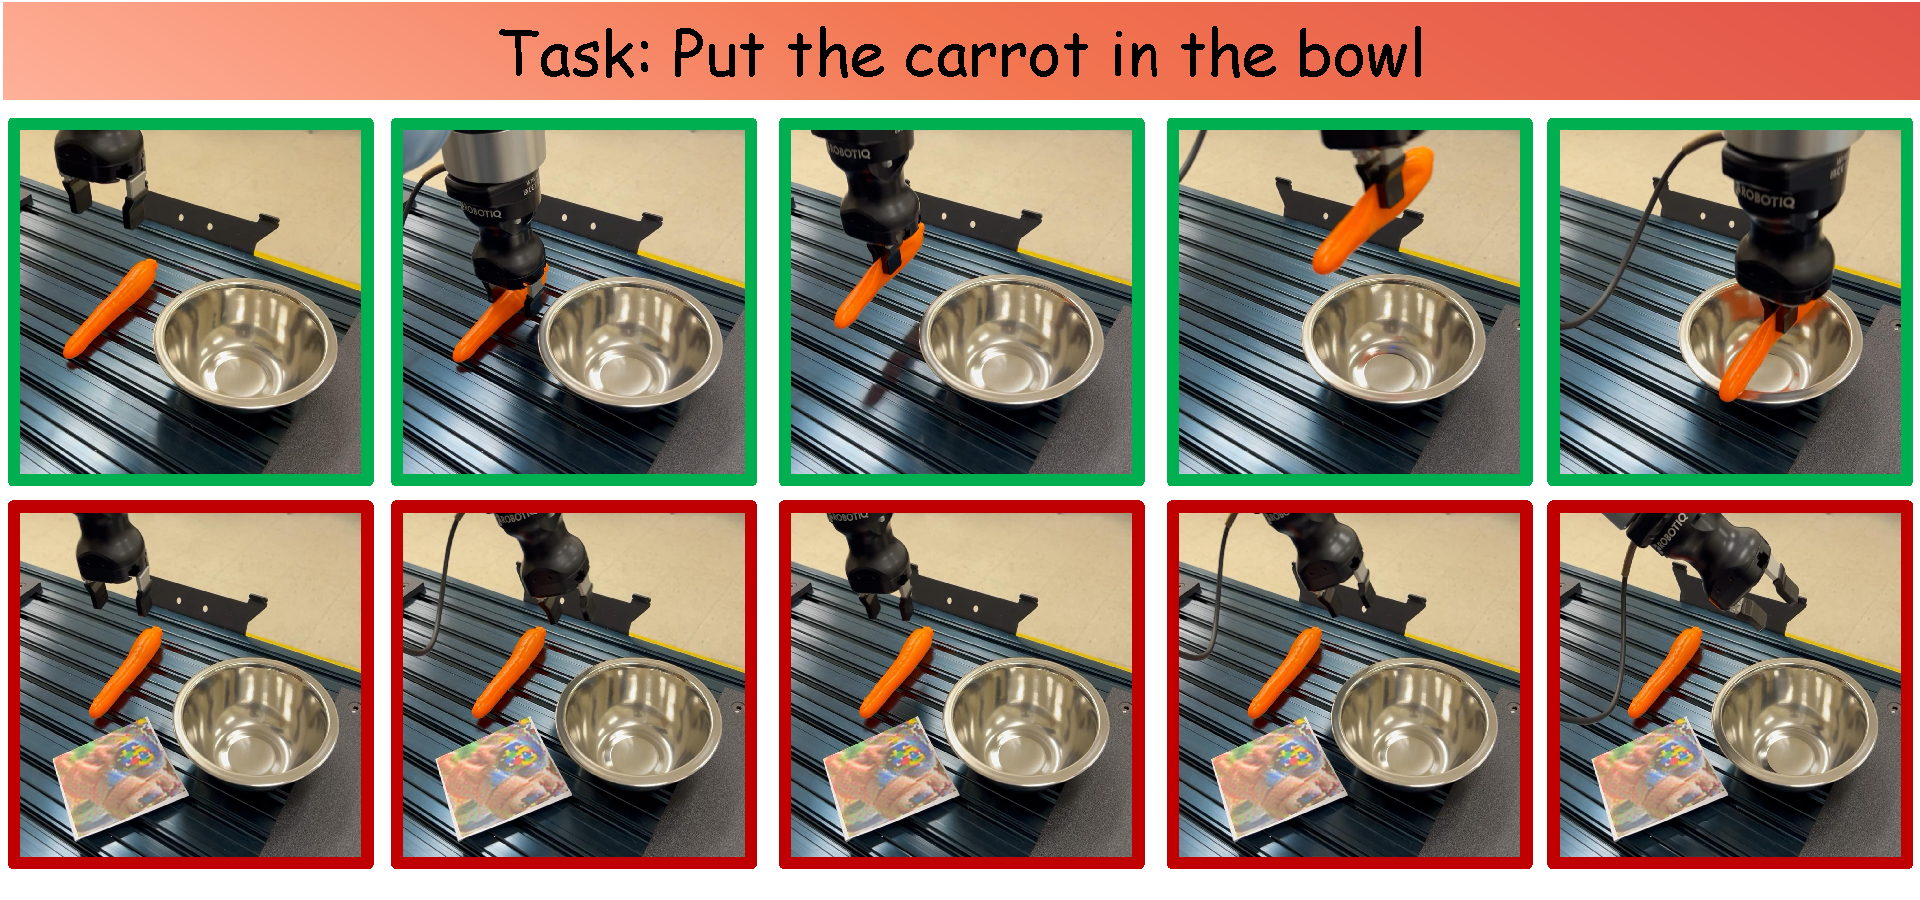
\includegraphics[width=0.88\linewidth]{images/physcialworld.pdf}
    \vspace{-10pt}
    \caption{\textbf{物理世界中的定性结果}。第一行/第二行分别展示了 \textcolor[HTML]{00B050}{良性} 与 \textcolor[HTML]{C00000}{对抗} 情况。}
    \label{fig:physcial}
    \vspace{-1.2em}
\end{figure}

\begin{figure}[htbp]
    \centering
    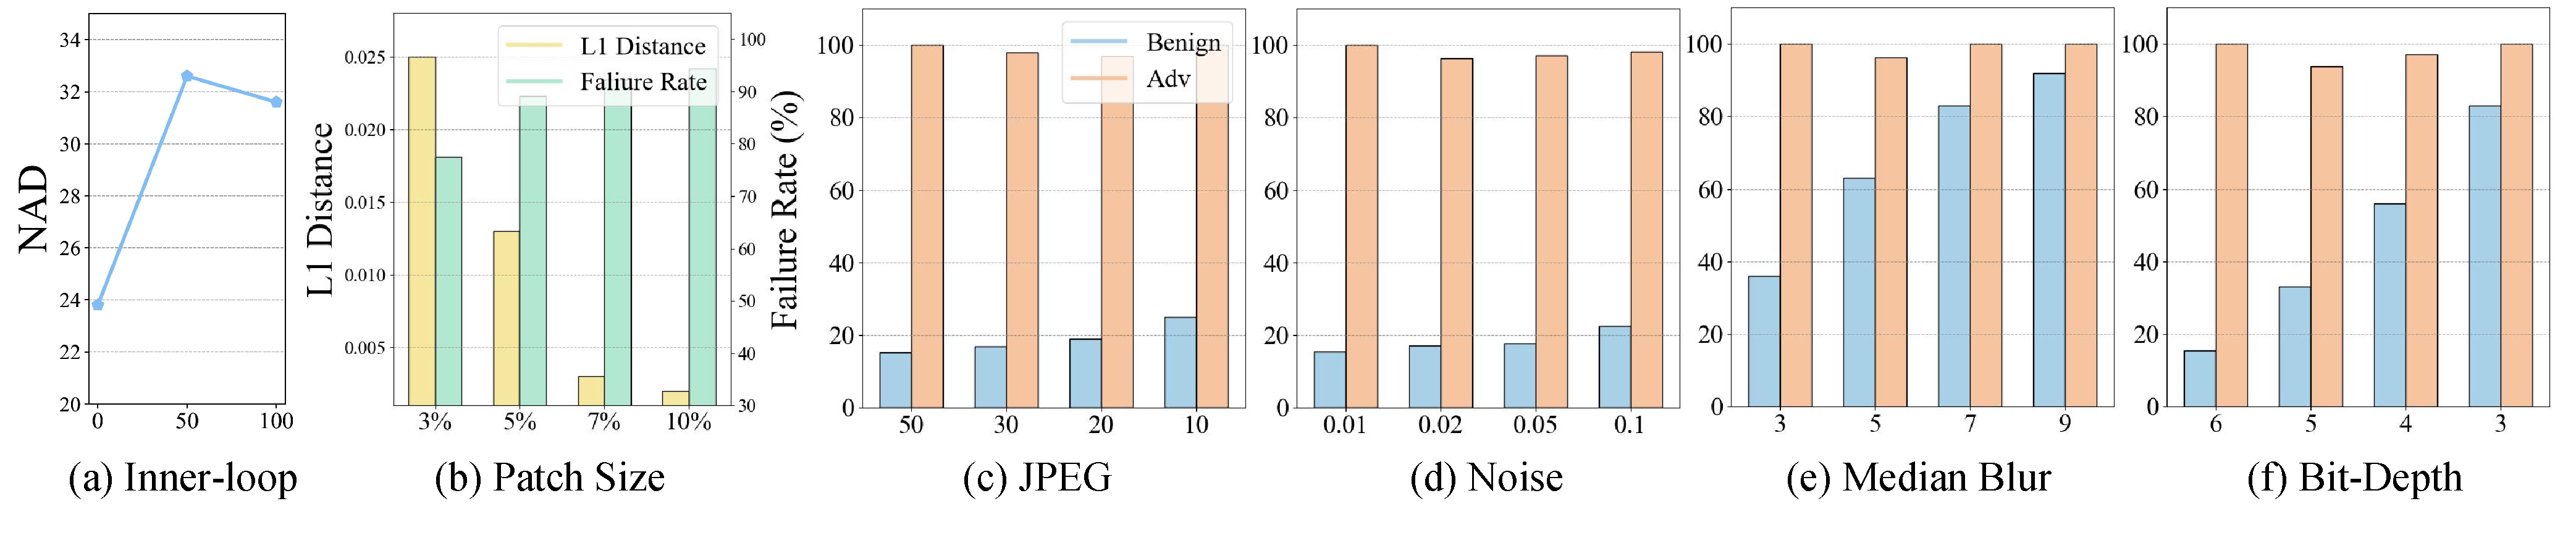
\includegraphics[width=0.95\linewidth]{images/defense.pdf}
    \vspace{-18pt}
    \caption{\textbf{内循环、补丁尺寸的影响与防御讨论}。图中展示了不同内循环步数对 UADA 中 NAD 的影响，以及不同补丁尺寸对以 DoF$_1$ 为攻击目标时 TMA 的 $L1$ 距离和失败率的影响。(a) 内循环的影响，(b) 补丁尺寸的影响，(c-f) 四种不同防御方法对失败率的影响。}
    \label{fig:patchsize}
    \vspace{-18pt}
\end{figure}

\textbf{真实世界表现。} 
除数字仿真结果外，我们还对所生成对抗补丁在真实世界场景中的表现进行了全面评估。评估包含三类不同任务上的 100 次试验：物体抓取、放置与操控。如图~\ref{fig:physcial} 所示，采用 UADA 生成的对抗补丁能够有效操纵机器人，攻击成功率超过 \textbf{43\%}。尽管这一成功率低于对应的数字世界表现（即，\textbf{100\%}），但它仍然表明本文补丁在物理世界应用中同样具有有效性，而且无需进一步适配。
更重要的是，我们观察到，在成功攻击中机器人出现的异常运动（与仿真场景相似）会对人类安全及周围环境带来显著风险。这一结果强调了 VLA 模型在真实世界应用中的严重威胁，与数字场景中的类似观察结论保持一致。

\subsection{诊断实验}\label{sec:diag}

\textbf{内循环的影响。} 
我们在图~\ref{fig:patchsize}(a) 中讨论内循环步数对模型表现的影响。结果表明，随着内循环步数增加，NAD 起初会提升。这是因为数据方差降低、梯度逐渐稳定。然而，当步数继续增大时，性能提升会放缓，同时训练时间显著增加。因此，我们选择内循环步数为 50，以在性能与规模之间取得平衡。 \\
\textbf{补丁尺寸的影响。} 
我们研究了不同补丁尺寸下 TMA 的表现，并在图~\ref{fig:patchsize}(b) 中报告了四个 LIBERO~\cite{LIBREO} 任务上的平均 FR。所考察的补丁尺寸为输入图像的 $[3\%, 5\%, 7\%, 10\%]$。
我们的发现表明，随着补丁尺寸增大，预测动作与目标动作之间的 $L_1$ 距离呈反比变化；同时，FR 也随之明显上升。这一趋势说明更大的补丁为攻击者提供了更大的优化空间去影响模型，与先前工作~\cite{cheng2024self,Zhang2022patchsize}的结论一致。

\subsection{鲁棒性评估} \label{sec:defense}

我们进一步考察现有防御策略~\cite{Gintare2016jpeg,Zhang2019noise,Xu2018medianblur}是否能够抵御 VLA 场景下的对抗样本。具体而言，我们应用了四种既有防御技术，并分别在图~\ref{fig:patchsize}(c-f) 中报告其对良性样本与对抗样本的 FR。结果表明，我们的对抗攻击能够绕过大多数防御策略。

\subsection{系统性讨论} \label{sec:sysdis}
\begin{figure}[t]
    \centering
    \begin{subfigure}{0.23\textwidth}
        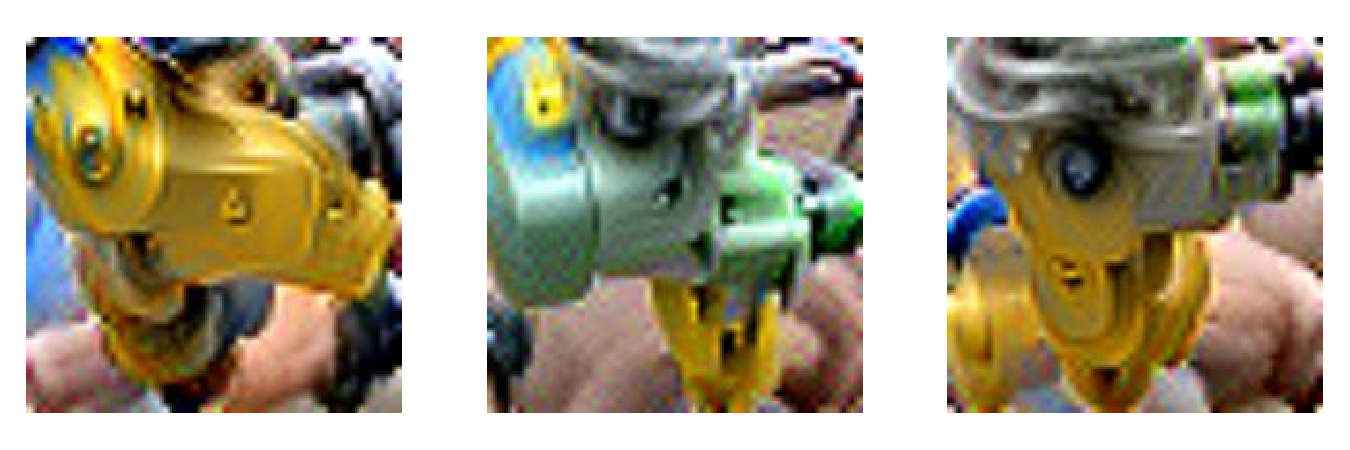
\includegraphics[width=\linewidth]{images/patchvis1.pdf}
        \caption{BridgeData V2~\cite{bridgev2}}
        \label{fig:vis1}
    \end{subfigure}
    \begin{subfigure}{0.23\textwidth}
        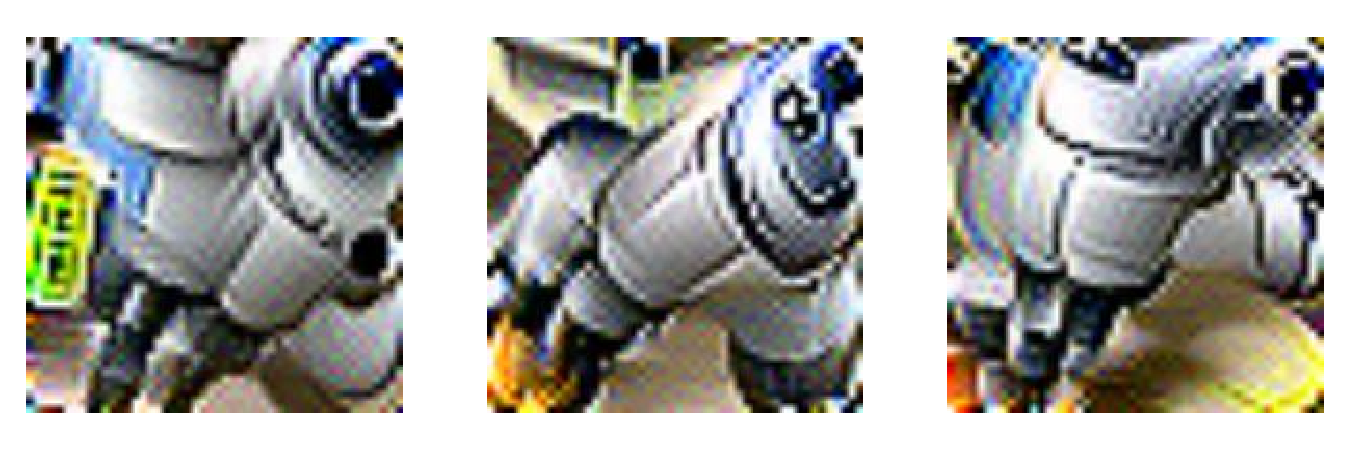
\includegraphics[width=\linewidth]{images/patchvis2.pdf}
        \caption{LIBERO~\cite{LIBREO}}
        \label{fig:vis2}
    \end{subfigure}
    \vspace{-8pt}
    \caption{\textbf{补丁可视化}。富含语义信息的补丁。}
    \label{fig:defensediscussion}
    \vspace{-1.5em}
\end{figure}
\textbf{补丁模式分析。} 
在图~\ref{fig:defensediscussion} 中，我们展示了针对一系列目标生成的对抗补丁。一个特别值得注意的现象是，其中一些补丁与机械臂的结构关节表现出惊人的相似性。鉴于这些补丁在外观上与机械臂高度相似，我们推测，当前训练范式下的基于 VLA 的模型往往只接触到有限范围的机器人系统，并且这些系统运行在受限的摄像头视角中。这种受限的透视摄像机位姿可能会无意中诱导一种表征偏置，使得对抗扰动在欺骗当前受害模型时，会与训练机器人外观中的显著结构特征相对齐。
考虑到这些补丁具有模型特异性，并反映了训练环境中的空间和视觉模式，我们有充分理由担忧，它们可能会削弱基于 VLA 模型在物理世界部署中的泛化能力与鲁棒性。 \\
\textbf{可能的防御策略。}
本文工作表明，为了成功抵御我们的攻击，基于 VLA 模型的训练策略亟需发生范式转变。具体而言，未来方法可以引入更多涉及复杂多机器人交互的训练场景，以缓解当前补丁偏置。另一种可能的解决方案是利用机械臂物理结构中的逻辑关系来估计各关节的真实位置。通过识别那些偏离物理约束的关节位置预测，我们可以剔除不合理的对抗样本，即便这些样本在外观上与真实关节相似。



\backmatter
\input{misc/1_conclusion.tex}
%%
% BIThesis 本科毕业设计论文翻译模板 —— 参考文献
%%

\begin{bibprint}

\printbibliography[heading=none]

\end{bibprint}

%%
% BIThesis 本科毕业设计论文翻译模板 —— 附录
%%

\begin{appendices}
\end{appendices}


\end{document}
